% \section*{Part 2}

% \begin{enumerate}
 
%     \item \textbf{Interference behavior}
%     \begin{enumerate}

% %%%%%%%%%%%%%%%%%%%%%%%%%%%%%%%%%%%%%%%%%%%
% %%% QUESTION 2.1A

%         \item Fill in the following table with the normalized execution time of each batch job with each source of interference. The execution time should be normalized to the job’s execution time with no interference. Round the normalized execution time to 2 decimal places. Color-code each cell in the table as follows: {\color{Green}\textbf{green}} if the normalized execution time is less than or equal to 1.3, {\color{YellowOrange}\textbf{orange}} if the normalized execution time is over 1.3 and less or equal to 2, and {\color{Red}\textbf{red}} if the normalized execution time is greater than 2. The coloring of the first three cells is given as an example of how to use the cell coloring command.   

%         % Fill in this table with your results and color the cells accordingly with the \cellcolor{color} command
% \begin{center}
% \begin{tabular}{ |c|c|c|c|c|c|c|c| } 
% \hline
%  \textbf{Workload} & \texttt{\textbf{none}} & \texttt{\textbf{cpu}} & \texttt{\textbf{l1d}} & \texttt{\textbf{l1i}} & \texttt{\textbf{l2}} & \texttt{\textbf{llc}} & \texttt{\textbf{memBW}}  \\
%  \hline\hline
% barnes         & 1.00 & \cellcolor{orange}1.48 & \cellcolor{orange}1.55 & \cellcolor{orange}1.92 & \cellcolor{orange}1.62 & \cellcolor{red}2.35 & \cellcolor{orange}1.58 \\  \hline
% blackscholes   & 1.00 & \cellcolor{Green}1.27 & \cellcolor{orange}1.31 & \cellcolor{orange}1.52 & \cellcolor{orange}1.34 & \cellcolor{orange}1.58 & \cellcolor{orange}1.38 \\  \hline
% canneal        & 1.00 & \cellcolor{Green}1.09 & \cellcolor{Green}1.14 & \cellcolor{Green}1.25 & \cellcolor{Green}1.17 & \cellcolor{orange}1.82 & \cellcolor{orange}1.35 \\  \hline
% freqmine       & 1.00 & \cellcolor{orange}1.88 & \cellcolor{Green}1.28 & \cellcolor{orange}1.93 & \cellcolor{Green}1.22 & \cellcolor{orange}1.79 & \cellcolor{orange}1.49 \\  \hline
% radix          & 1.00 & \cellcolor{Green}1.08 & \cellcolor{Green}1.03 & \cellcolor{Green}1.07 & \cellcolor{Green}1.02 & \cellcolor{orange}1.72 & \cellcolor{Green}0.99 \\  \hline
% streamcluster  & 1.00 & \cellcolor{Green}1.23 & \cellcolor{Green}1.28 & \cellcolor{orange}1.54 & \cellcolor{Green}1.26 & \cellcolor{orange}1.95 & \cellcolor{Green}1.29 \\  \hline
% vips           & 1.00 & \cellcolor{orange}1.60 & \cellcolor{orange}1.73 & \cellcolor{orange}1.75 & \cellcolor{orange}1.66 & \cellcolor{orange}1.81 & \cellcolor{orange}1.69 \\  \hline
% \end{tabular}
% \end{center}
% % \begin{figure}[H]
% %     \centering
% %     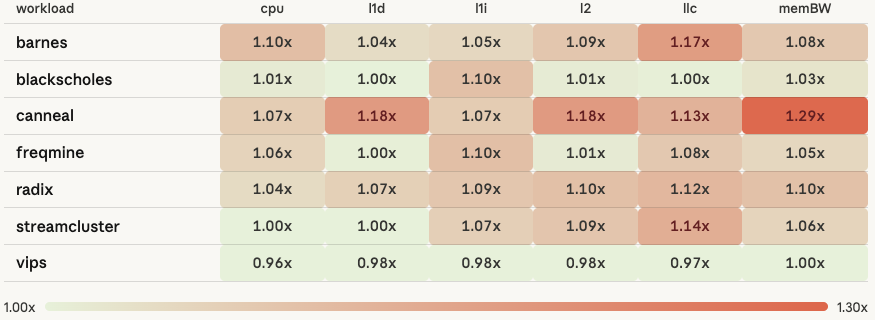
\includegraphics[width=0.75\linewidth]{figures/heatmap.png}
% %     \caption{Heatmap}
% %     \label{fig:placeholder}
% % \end{figure}


% %%%%%%%%%%%%%%%%%%%%%%%%%%%%%%%%%%%%%%%%%%%
% %%% QUESTION 2.1B

% \item Explain what the interference profile table tells you about the resource requirements for each job. Give your reasoning behind these resource requirements based on the functionality of each job.

% \textbf{Answer:}

% \begin{itemize}

% \item \texttt{barnes:} Barnes is highly sensitive to LLC interference (2.35x slowdown) and shows strong sensitivity to L1i and L2 interference as well.

% \textit{Explanation:} Barnes performs irregular tree traversals in the Barnes-Hut algorithm. The pointer-based octree structure generates non-contiguous memory accesses, which heavily stress the last-level cache. Frequent instruction and data movement also explains the sensitivity to L1i and L2. This workload is clearly memory-hierarchy bound.

% \item \texttt{blackscholes:} Blackscholes shows moderate sensitivity to LLC and instruction-cache interference (up to 1.58x), but remains relatively stable under other sources.

% \textit{Explanation:} The computation consists of independent floating-point operations on a regular dataset. The workload is mostly compute-bound, but instruction and higher-level cache interference can slightly degrade performance due to code and data eviction.

% \item \texttt{canneal:} Canneal is particularly sensitive to LLC (1.82x) and memory bandwidth interference (1.35x), with mild sensitivity to lower cache levels.

% \textit{Explanation:} Simulated annealing involves frequent random memory accesses over a large netlist. The working set exceeds lower cache sizes, making the workload dependent on LLC capacity and memory bandwidth. This indicates a memory-intensive workload.

% \item \texttt{freqmine:} Freqmine shows strong sensitivity to CPU (1.88x), L1i (1.93x), and LLC (1.79x) interference.

% \textit{Explanation:} The FP-growth algorithm has irregular control flow and heavy branching, stressing the instruction cache. Pointer-based tree traversals also pressure the LLC. The strong CPU sensitivity suggests significant computational work combined with memory pressure.

% \item \texttt{radix:} Radix is mostly sensitive to LLC interference (1.72x) while remaining relatively stable under other interference types.

% \textit{Explanation:} Radix sort processes a very large dataset across multiple passes. Since the dataset far exceeds cache capacity, it relies on streaming memory access. LLC interference increases cache misses and DRAM traffic, explaining the slowdown.

% \item \texttt{streamcluster:} Streamcluster is sensitive to LLC (1.95x) and moderately affected by L1i and L2 interference.

% \textit{Explanation:} The algorithm repeatedly computes distances between points and cluster centers. The working set does not fit entirely in lower-level caches, making it dependent on higher-level cache capacity. LLC interference causes repeated memory reloads.

% \item \texttt{vips:} Vips shows consistent sensitivity across all interference types (around 1.6–1.8x), without a single dominant bottleneck.

% \textit{Explanation:} Image processing involves large data arrays and continuous data movement. Although access patterns are regular, the dataset is large enough to stress caches and memory bandwidth. The workload therefore suffers under both compute and memory interference.

% \end{itemize}

% %%%%%%%%%%%%%%%%%%%%%%%%%%%%%%%%%%%%%%%%%%%
% %%% QUESTION 2.1C
%  \item Which jobs (if any) seem like good candidates to collocate with memcached from Part 1, without violating the SLO of 2 ms P95 latency at 40K QPS? Explain why.

% \textbf{Answer:}

% Based on the interference profiles from Part 2 and the memcached sensitivity results from Part 1, \texttt{blackscholes} is the safest candidate for collocation with memcached. 

% From Part 1, memcached was particularly sensitive to CPU and instruction-cache interference, as these directly increased tail latency. \texttt{blackscholes} shows only mild slowdowns across all interference sources ($\leq$1.58x) and does not heavily stress CPU or lower-level caches. Since it is mostly compute-bound with regular access patterns and a small working set, it is unlikely to significantly impact memcached latency at 40K QPS.

% \texttt{radix} and \texttt{canneal} may be borderline candidates. Although they are not heavily CPU-sensitive, they show noticeable LLC sensitivity, which could affect memcached if both workloads compete for shared cache capacity. Careful core placement would be required.

% In contrast, \texttt{barnes}, \texttt{freqmine}, \texttt{streamcluster}, and \texttt{vips} are poor candidates. They exhibit strong sensitivity to CPU, instruction cache, or LLC interference (in some cases close to or above 2x slowdown). Since memcached relies on fast instruction execution and low-latency memory access, colocating it with these workloads would likely increase tail latency and risk violating the 2 ms SLO.
% %%%%%%%%%%%%%%%%%%%%%%%%%%%%%%%%%%%%%%%%%%%
% %%% QUESTION 2.2A
% \newpage
%         \item Plot a line graph with speedup as the y-axis (normalized time to the single thread config, $\textrm{Time}_1$ / $\textrm{Time}_n)$ vs. number of threads on the x-axis (1, 2, 4 and 8 threads - see the project description for more details). Pay attention to the readability of your graph. % it will be a part of your grade.

%         \textbf{Answer:} % Here you place your solution.
%         \begin{figure}[H]
%             \centering
%             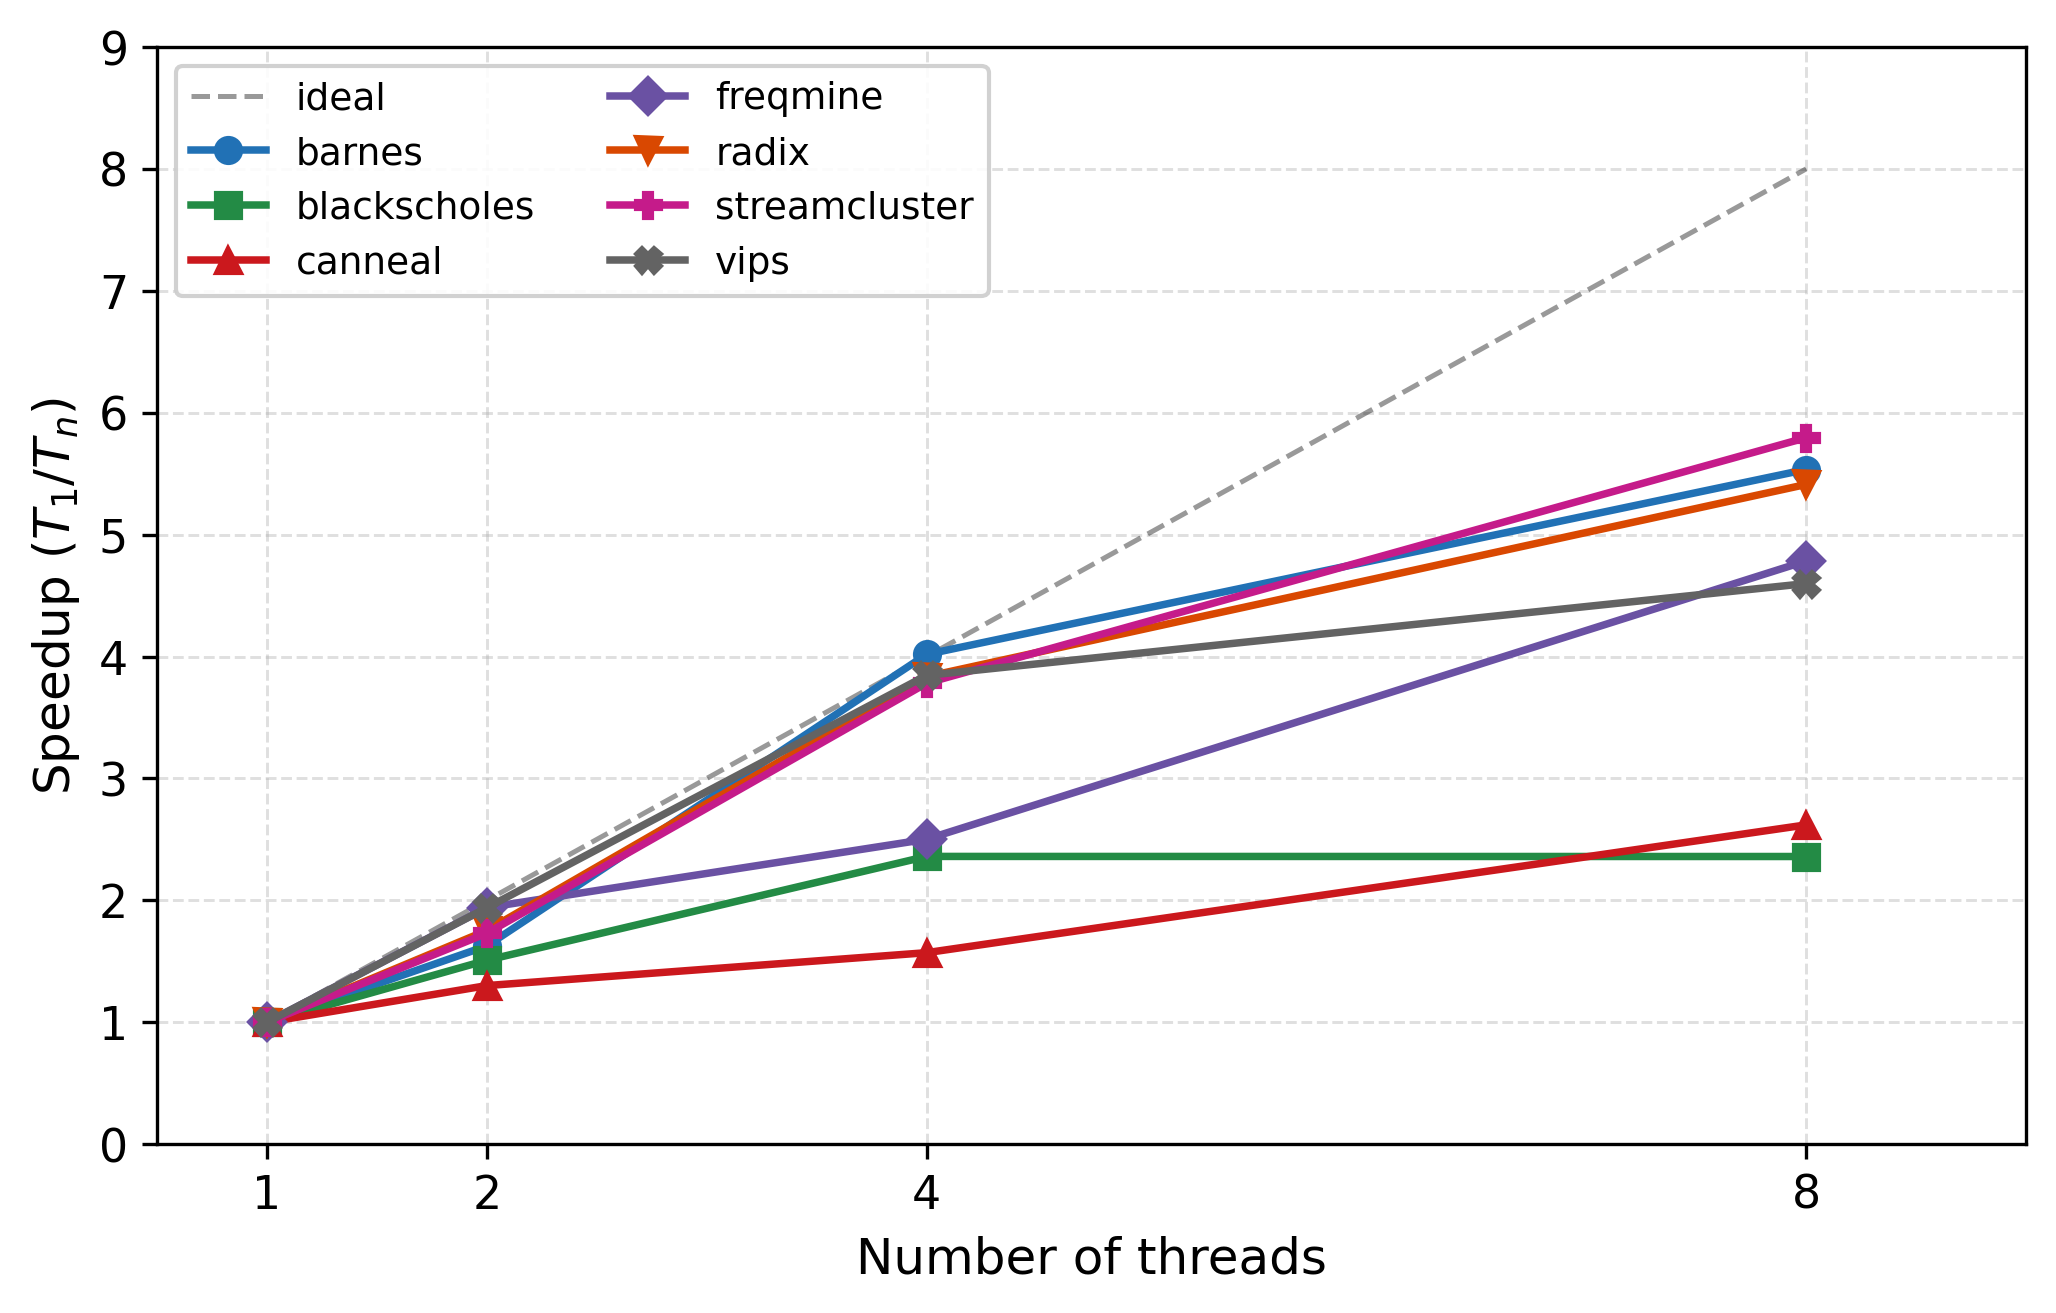
\includegraphics[width=0.85\textwidth]{Project Template/figures/part2b_speedup.png}
%         \end{figure}


        
% %%%%%%%%%%%%%%%%%%%%%%%%%%%%%%%%%%%%%%%%%%%
% %%% QUESTION 2.2B

%         \item Briefly discuss the scalability of each job: e.g., linear/sub-linear/super-linear. Do the applications gain significant speedup with the increased number of threads? Explain what you consider to be ``significant''.
%         \textbf{Answer:}

%         We define a speedup as \textbf{significant} if it is at least 1.5$\times$ relative to the single-thread baseline, i.e., a speedup at 8 threads of $\geq$1.5$\times$. We consider scalability \textbf{good} when parallel efficiency (speedup$/n$) exceeds 60\%, \textbf{moderate} between 30--60\%, and \textbf{poor} below 30\%.

%         \begin{itemize}
%             \item \texttt{barnes:} Sub-linear but good scalability. Speedup reaches 1.63$\times$ at 2 threads, 4.02$\times$ at 4 threads, and 5.53$\times$ at 8 threads (parallel efficiency: 69\%). The speedup is significant: at 8 threads the job runs in 28.7s versus 158.7s single-threaded. The sub-linear behavior is expected because the Barnes-Hut tree must be rebuilt and shared across threads, introducing synchronization overhead that grows with thread count.
%             \\

%             \item \texttt{blackscholes:} Sub-linear with poor scalability beyond 2 threads. Speedup grows to 1.51$\times$ at 2 threads and 2.36$\times$ at 4 threads, but stalls completely at 8 threads (also 2.36$\times$, parallel efficiency: 30\%). The speedup is \textbf{not significant} at 8 threads, as doubling the thread count from 4 to 8 yields zero benefit. This plateau suggests that the bottleneck shifts to memory bandwidth: the native dataset is 400 MB (10M options), and once all 4 threads saturate the memory bus, adding more threads provides no gain.
%             \\

%             \item \texttt{canneal:} Sub-linear with poor scalability. Speedup is only 1.30$\times$ at 2 threads, 1.57$\times$ at 4 threads, and 2.62$\times$ at 8 threads (parallel efficiency: 33\%). The speedup is \textbf{not significant} relative to the thread count. Canneal's simulated annealing requires threads to share a large netlist (2.5M elements) and perform random read-write accesses to common locations. This creates heavy contention on shared cache lines and causes frequent cache invalidations between threads (false sharing), severely limiting parallel scalability.
%             \\

%             \item \texttt{freqmine:} Sub-linear but moderate scalability with an unusual pattern. Speedup reaches 1.94$\times$ at 2 threads but then grows slowly to 2.50$\times$ at 4 threads, before jumping to 4.78$\times$ at 8 threads (parallel efficiency: 60\%). The speedup is significant overall. The non-monotonic behavior — where going from 2 to 4 threads gives less benefit than going from 4 to 8 — suggests that freqmine's FP-growth tree partitioning becomes more efficient at higher thread counts once the per-thread working sets fit better in the distributed caches.
%             \\

%             \item \texttt{radix:} Sub-linear but good scalability. Speedup reaches 1.75$\times$ at 2 threads, 3.84$\times$ at 4 threads, and 5.41$\times$ at 8 threads (parallel efficiency: 68\%). The speedup is significant and among the best in the suite. Radix sort parallelizes well because each thread can independently sort its partition of the data; the main bottleneck is the synchronization barrier between passes, which is unavoidable but scales relatively well.
%             \\

%             \item \texttt{streamcluster:} Sub-linear but good scalability, the best in the suite. Speedup reaches 1.73$\times$ at 2 threads, 3.78$\times$ at 4 threads, and 5.80$\times$ at 8 threads (parallel efficiency: 72\%). The speedup is significant. Streamcluster parallelizes the distance computations across threads, which is an embarrassingly parallel operation: each thread computes distances for its subset of points independently, with minimal synchronization needed only when updating cluster centers.
%             \\

%             \item \texttt{vips:} Sub-linear but good scalability. Speedup reaches 1.94$\times$ at 2 threads, 3.85$\times$ at 4 threads, and 4.60$\times$ at 8 threads (parallel efficiency: 57\%). The speedup is significant up to 4 threads, but shows diminishing returns at 8 threads. Vips parallelizes image processing across rows of the image; the streaming, sequential access pattern that made it interference-resilient in Part 2a also limits parallelism at high thread counts, as the memory bus becomes saturated when 8 threads simultaneously stream through the 18,000$\times$18,000 pixel image.
%             \\
%         \end{itemize}

% \newpage
